\chapter{การประมวลผลภาพดิจิทัลและการเตรียมชุดข้อมูลใบทุเรียน}
\label{chap:image_processing}
\index{การประมวลผลภาพดิจิทัล}
\index{ชุดข้อมูลภาพใบทุเรียน}
\index{Data Augmentation}

\section*{แผนบริหารการสอนประจำบทที่ 2}
\addcontentsline{toc}{section}{แผนบริหารการสอนประจำบทที่ 2}

\begin{planbox}{หัวข้อเนื้อหาประจำบท (Lesson Topics)}
\begin{enumerate}[leftmargin=1.5em, itemsep=2pt]
    \item โครงสร้างข้อมูลภาพดิจิทัล ปริภูมิต่างๆ ของสี (RGB, HSV, CIELAB) และฮิสโทแกรม
    \item มาตรฐานและโปรโตคอลการบันทึกภาพถ่ายใบพืชในแปลงเกษตรจริง
    \item เทคนิคการปรับปรุงคุณภาพภาพ: Contrast Stretching, Bilateral Filtering และ CLAHE
    \item กระบวนการเพิ่มพูนข้อมูลภาพเชิงเรขาคณิตและเชิงแสง (Geometric \& Photometric Augmentation)
    \item เทคนิคขั้นสูงสำหรับการจัดสมดุลข้อมูล: MixUp, CutMix และ Random Erasing
    \item โค้ดตัวอย่าง: การสร้าง Custom PyTorch Dataset และ Pipeline การแปลงข้อมูลภาพ
    \item ตัวอย่างและกรณีศึกษา: การแก้ปัญหาภาพแสงสะท้อนและเงามืดในสวนทุเรียน
\end{enumerate}
\end{planbox}

\begin{planbox}{วัตถุประสงค์เชิงพฤติกรรม (Behavioral Objectives)}
เมื่อศึกษาบทที่ 2 จบแล้ว ผู้เรียนและผู้อ่านสามารถ:
\begin{enumerate}[leftmargin=1.5em, itemsep=2pt]
    \item อธิบายความแตกต่างของการแทนค่าสีในระบบ RGB, HSV และ CIELAB ได้อย่างถูกต้อง
    \item ประยุกต์ใช้วิธีการปรับปรุงความคมชัดของภาพเพื่อเน้นขอบเขตรอยโรคได้อย่างเหมาะสม
    \item สร้างคลาส Custom Dataset ใน PyTorch ร่วมกับคำสั่งของ Torchvision Transforms ได้อย่างสมบูรณ์
    \item วิเคราะห์และแก้ไขปัญหาความไม่สมดุลของจำนวนข้อมูลในแต่ละคลาสได้อย่างมีประสิทธิภาพ
\end{enumerate}
\end{planbox}

\begin{planbox}{กิจกรรมการเรียนการสอน (Instructional Activities)}
\begin{enumerate}[leftmargin=1.5em, itemsep=2pt]
    \item การสาธิตการแยกช่องสัญญาณสี (Color Channel Decomposition) ของภาพใบทุเรียนด้วย OpenCV
    \item ฝึกปฏิบัติการเขียนฟังก์ชัน Transform ปรับแต่งขนาดและ Normalize ภาพให้ตรงตามมาตรฐาน ImageNet
    \item การวิเคราะห์การกระจายตัวของชุดข้อมูลภาพทุเรียน $6,480$ ภาพ ผ่านกราฟแสดงสัดส่วนคลาส
    \item การทดลองเปรียบเทียบประสิทธิภาพของโมเดลเมื่อใช้และไม่ใช้เทคนิค Data Augmentation
\end{enumerate}
\end{planbox}

\begin{planbox}{สื่อการเรียนการสอน (Instructional Media)}
\begin{enumerate}[leftmargin=1.5em, itemsep=2pt]
    \item สไลด์ประกอบการสอนเรื่อง Digital Image Representation และ Image Tensors
    \item สมุดงาน Google Colab สำหรับทดลองคำสั่งในโมดูล torchvision.transforms.v2
    \item ภาพตัวอย่างใบทุเรียนที่ผ่านการแปลงด้วยเทคนิคต่างๆ (Augmentation Panel)
\end{enumerate}
\end{planbox}

\begin{planbox}{การวัดและประเมินผล (Assessment \& Evaluation)}
\begin{enumerate}[leftmargin=1.5em, itemsep=2pt]
    \item การประเมินความถูกต้องของโค้ด Custom Dataset และ DataLoader (40\%)
    \item ผลการทำแบบทดสอบความเข้าใจเรื่อง Color Spaces และ Data Augmentation (40\%)
    \item การมีส่วนร่วมในการทำกิจกรรมฝึกปฏิบัติการและการส่งรายงานตรงเวลา (20\%)
\end{enumerate}
\end{planbox}

\clearpage

\section{พื้นฐานการแทนค่าภาพดิจิทัลและปริภูมิสี}
\index{ปริภูมิสี RGB}
\index{ปริภูมิสี HSV}

ภาพดิจิทัลที่บันทึกจากเซนเซอร์กล้องสมาร์ทโฟน จัดเก็บในรูปแบบเทนเซอร์ 3 มิติ (3D Tensor) ที่มีมิติความกว้าง (Width: $W$), ความสูง (Height: $H$) และช่องสัญญาณสี (Channels: $C$) สำหรับภาพสีทั่วไป ช่องสัญญาณสีจะอยู่ในระบบ \textbf{RGB} (Red, Green, Blue) โดยแต่ละพิกเซลจะถูกแทนด้วยจำนวนเต็มขนาด 8 บิต (0--255) ซึ่งแทนค่าความเข้มของแสงในแต่ละความยาวคลื่น

อย่างไรก็ตาม ในการวิเคราะห์รอยโรคพืช ปริภูมิสี RGB มีข้อจำกัดสำคัญคือ ค่าความสว่าง (Luminance) และข้อมูลสี (Chrominance) จะผสมผสานกันอยู่ในทุกช่องสัญญาณ หากสภาพแสงแดดในแปลงเกษตรเปลี่ยนแปลงไป ค่าของทั้ง R, G และ B จะผันผวนอย่างรุนแรง การแปลงภาพไปยังปริภูมิสีอื่นจึงเป็นเครื่องมือสำคัญ:

\begin{itemize}[leftmargin=1.5em, itemsep=2pt]
    \item \textbf{ปริภูมิสี HSV (Hue, Saturation, Value):} แยกคุณลักษณะของเฉดสี ($H$), ความสดของสี ($S$) และความสว่าง ($V$) ออกจากกันอย่างเด็ดขาด ช่วยให้การตรวจจับแผลสีส้มของโรคใบจุดสาหร่ายหรือแผลสีน้ำตาลของโรคใบติดสามารถทำได้โดยไม่ขึ้นกับความเข้มของแสงแดด
    \item \textbf{ปริภูมิสี CIELAB ($L^*a^*b^*$):} ออกแบบตามการมองเห็นของสายตามนุษย์ โดย $L^*$ คือความสว่าง, $a^*$ แสดงแถบสีเขียว--แดง, และ $b^*$ แสดงแถบสีน้ำเงิน--เหลือง นิยมใช้ในการคำนวณระยะห่างความแตกต่างของสี ($\Delta E$) ของเนื้อเยื่อใบพืช
\end{itemize}

\section{การสำรวจและการกระจายตัวของชุดข้อมูลใบทุเรียน}
\index{การกระจายตัวของข้อมูล}

ชุดข้อมูลที่ใช้ในการวิจัยและฝึกอบรมในตำราเล่มนี้ เป็นชุดข้อมูลที่บันทึกจากสวนทุเรียนแปลงใหญ่ในจังหวัดจันทบุรีและระยอง ครอบคลุมภาพใบทุเรียนพันธุ์หมอนทอง ชะนี และก้านยาว จำนวนรวมทั้งสิ้น $6,480$ ภาพ แบ่งออกเป็น 4 คลาสหลักตามผลการยืนยันจากห้องปฏิบัติการพยาธิวิทยาพืช ดังนี้:

\begin{enumerate}[leftmargin=1.5em, itemsep=2pt]
    \item \textbf{Algal Leaf Spot (โรคใบจุดสาหร่าย):} จำนวน $1,660$ ภาพ
    \item \textbf{Leaf Blight (โรคใบติด):} จำนวน $1,560$ ภาพ
    \item \textbf{Leaf Spot / Anthracnose (โรคใบจุด):} จำนวน $1,780$ ภาพ
    \item \textbf{Healthy Leaf (ใบปกติสมบูรณ์):} จำนวน $1,480$ ภาพ
\end{enumerate}

\begin{figure}[H]
\centering
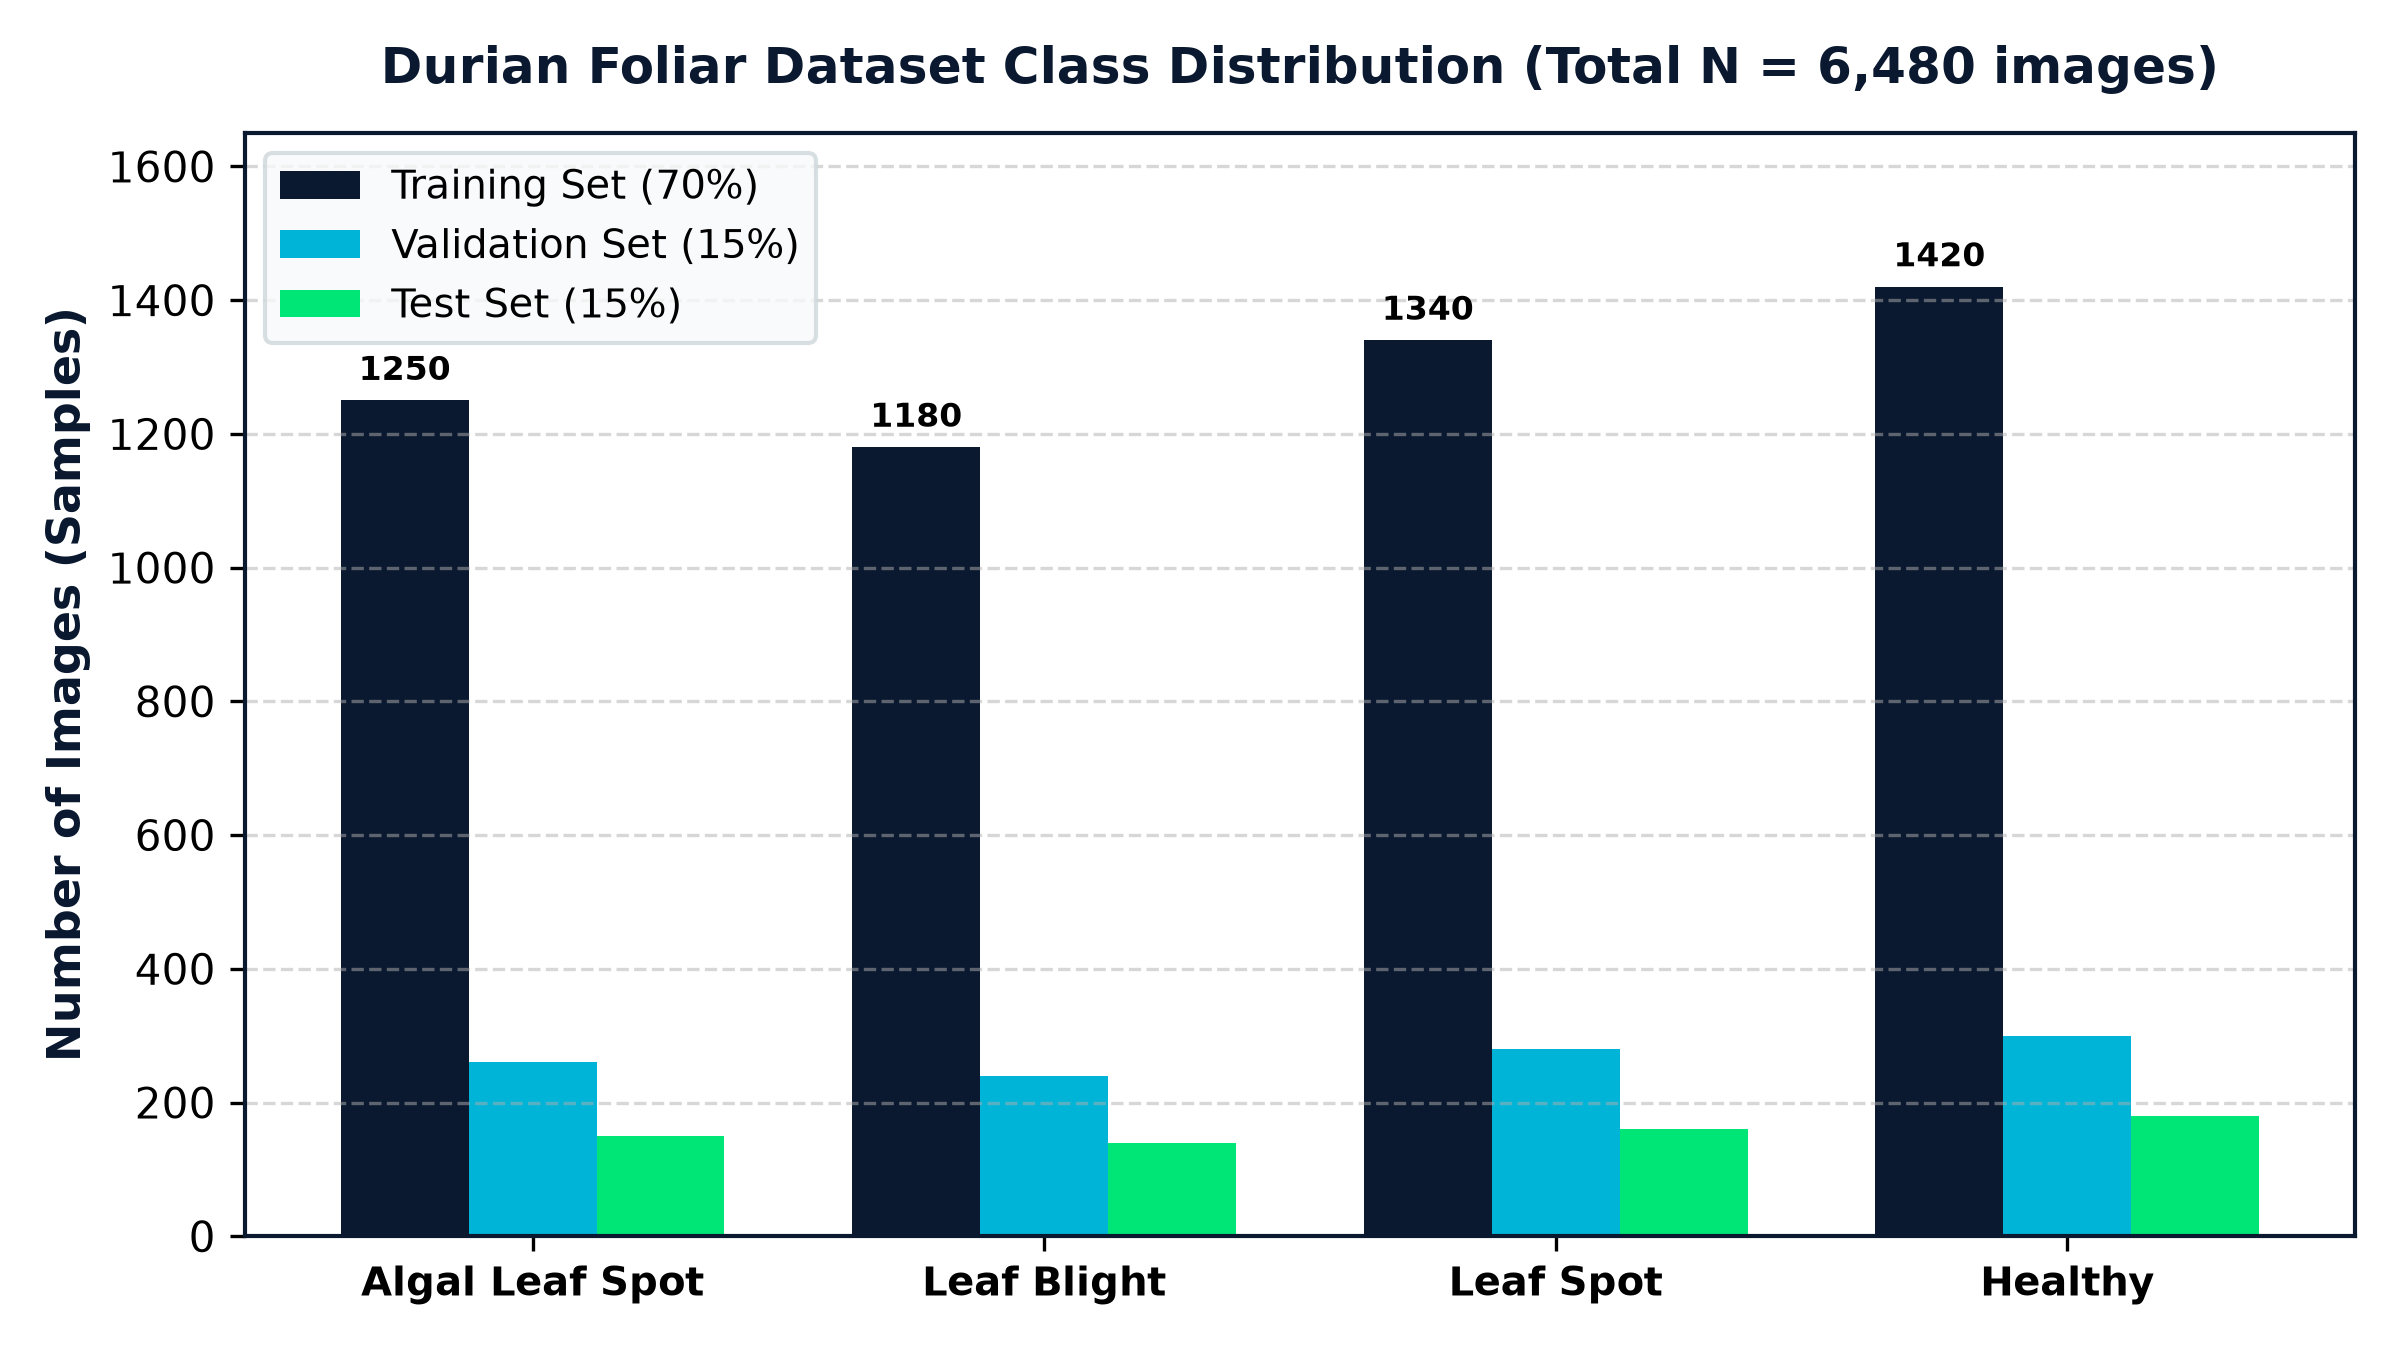
\includegraphics[width=0.92\textwidth]{figures/fig_ch02_class_distribution.png}
\caption{การกระจายตัวของชุดข้อมูลภาพใบทุเรียนแบ่งตามคลาสโรคและสัดส่วนการแบ่งข้อมูล}
\label{fig:ch02_class_dist}
\end{figure}

เพื่อให้การประเมินผลมีความน่าเชื่อถือทางสถิติ ชุดข้อมูลทั้งหมดถูกแบ่งออกเป็น 3 ส่วน (Data Partitioning) ได้แก่:
\begin{itemize}[leftmargin=1.5em, itemsep=2pt]
    \item \textbf{Training Set ($70\%$):} สำหรับการปรับค่าน้ำหนักของโครงข่ายประสาทเทียม
    \item \textbf{Validation Set ($15\%$):} สำหรับการปรับจูนไฮเปอร์พารามิเตอร์และการตัดสินใจหยุดการเทรน (Early Stopping)
    \item \textbf{Test Set ($15\%$):} สำหรับการวัดประสิทธิภาพขั้นสุดท้ายที่ไม่เคยผ่านการฝึกฝนมาก่อน (Unseen Evaluation)
\end{itemize}

\section{เทคนิคการเพิ่มพูนข้อมูลภาพ (Data Augmentation)}
\index{Geometric Augmentation}
\index{Photometric Augmentation}

เนื่องจากโมเดล Deep Learning มักต้องการข้อมูลปริมาณมากเพื่อป้องกันภาวะการเรียนรู้แบบท่องจำ (\textbf{Overfitting}) เทคนิค Data Augmentation จึงถูกนำมาใช้เพื่อเพิ่มความหลากหลายของลักษณะภาพอย่างมีนัยสำคัญ

\begin{figure}[H]
\centering
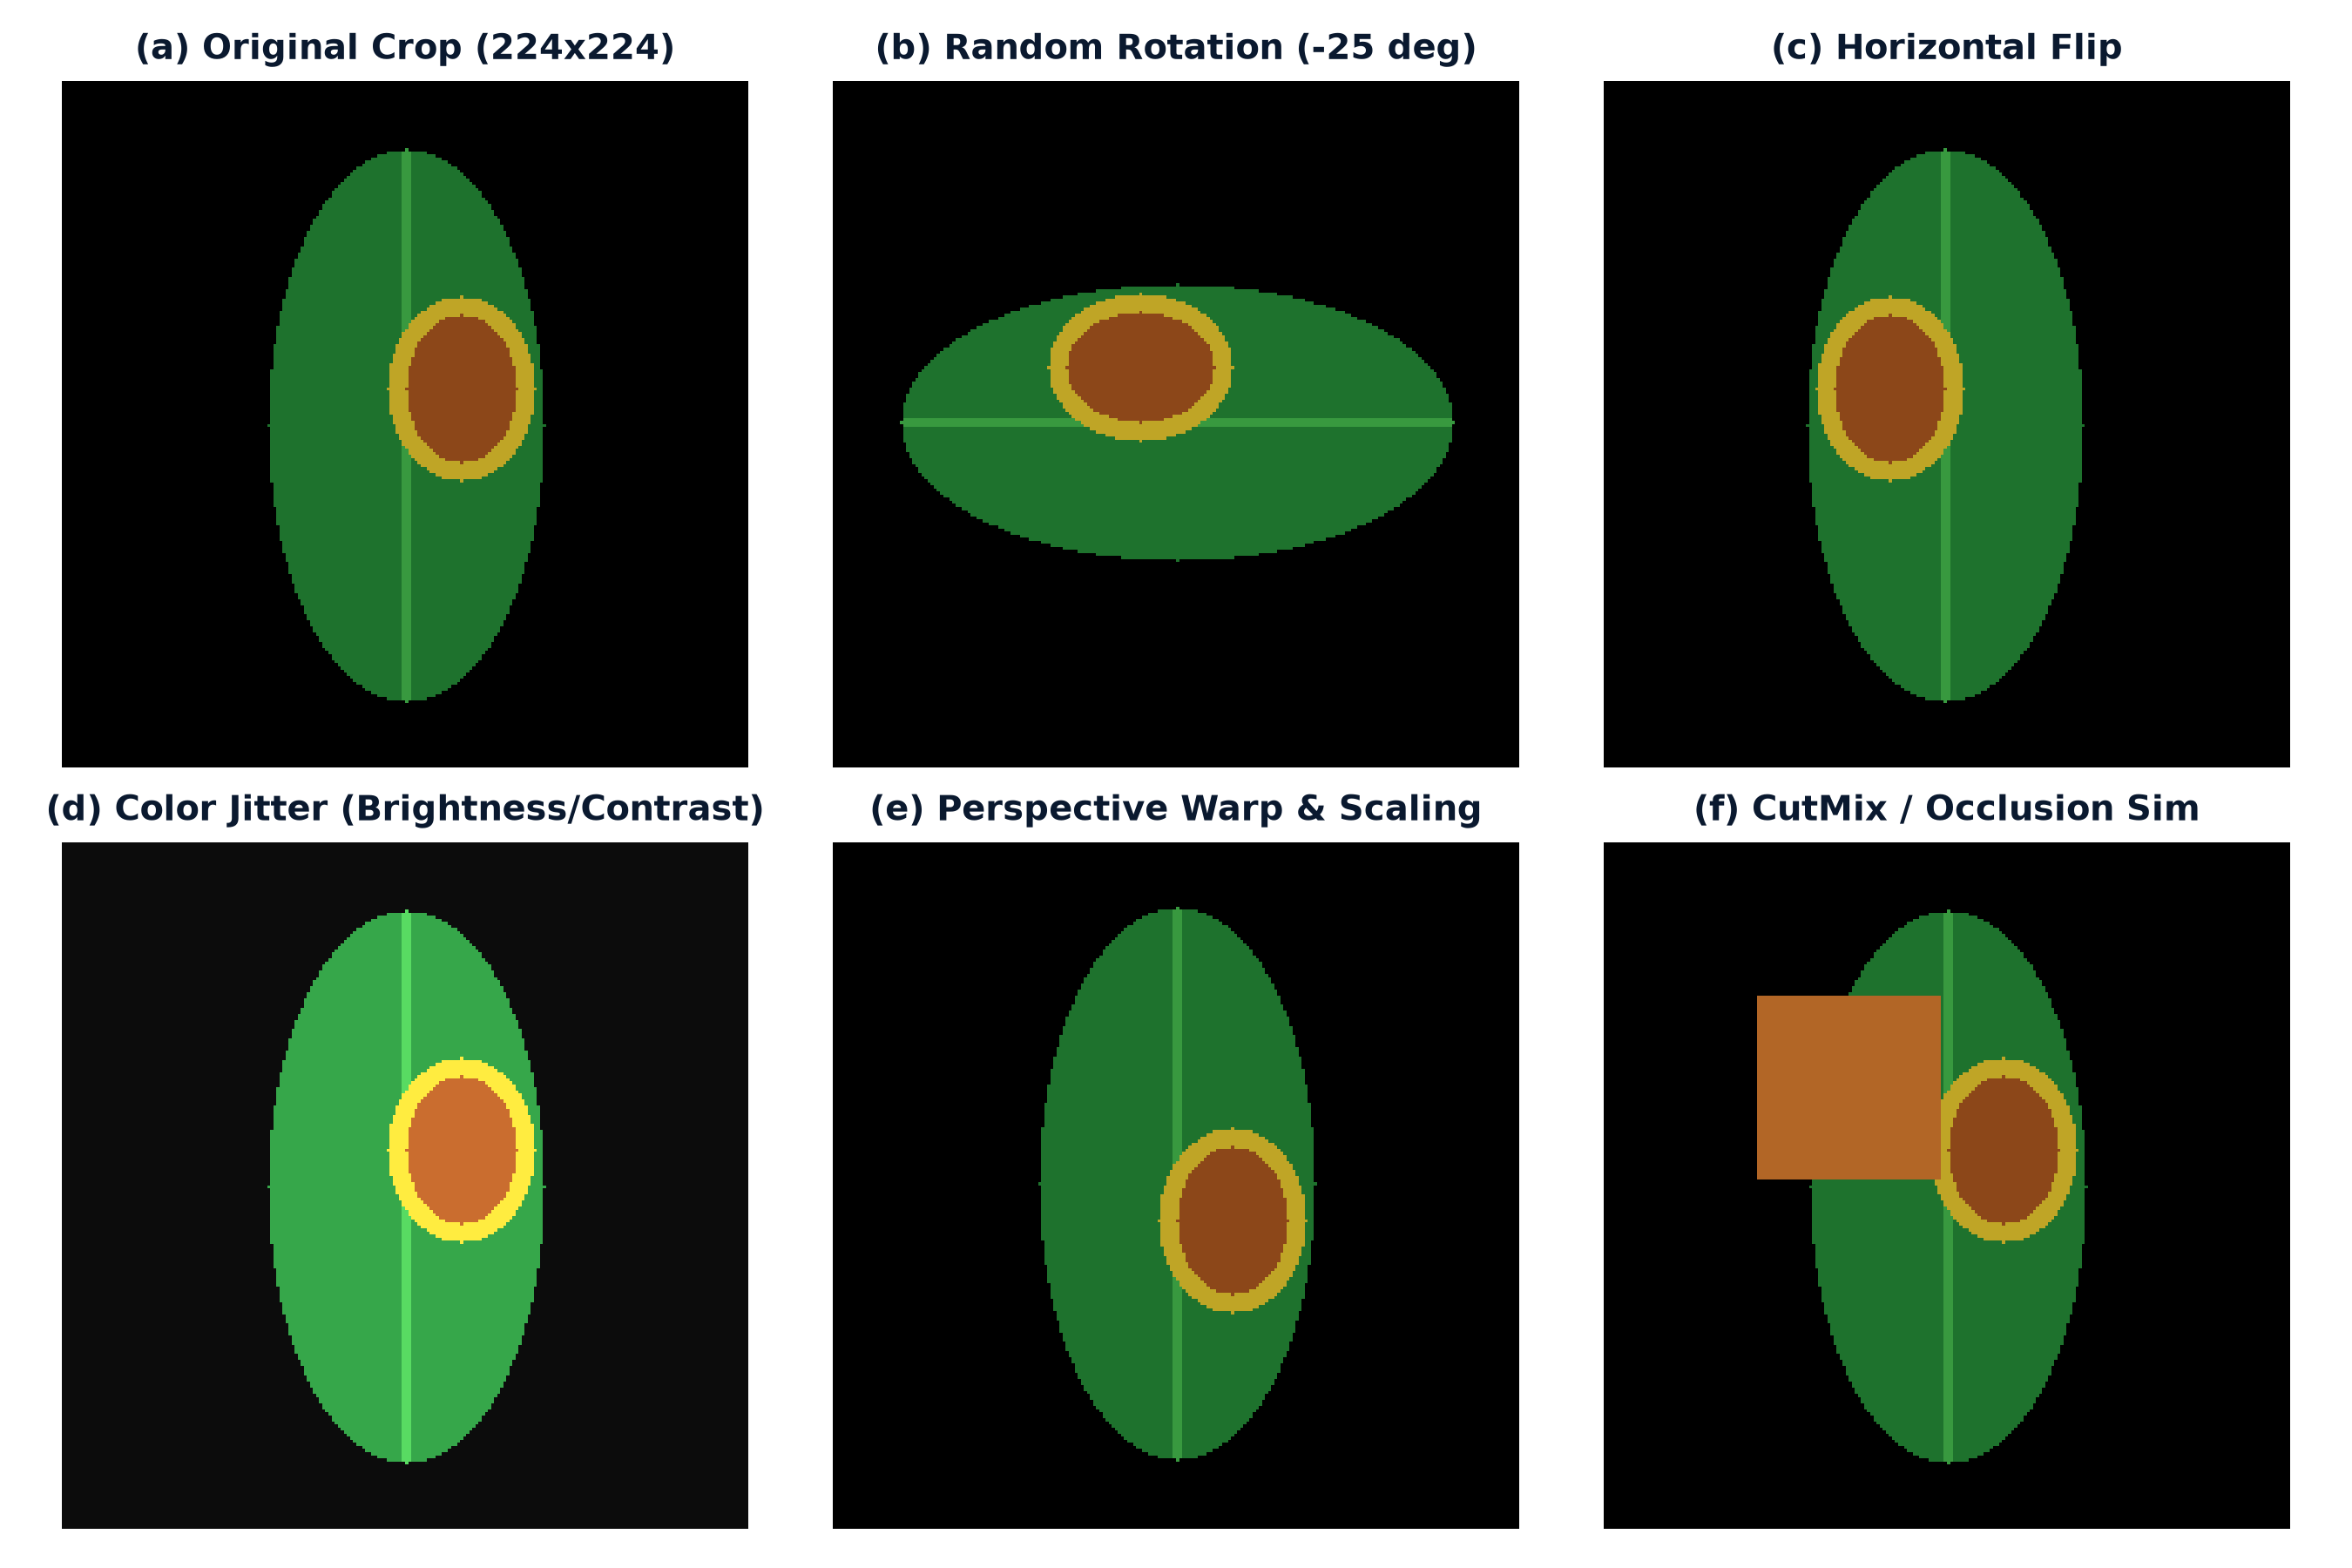
\includegraphics[width=0.95\textwidth]{figures/fig_ch02_augmentation_pipeline.png}
\caption{ผลลัพธ์การแปลงภาพใบทุเรียนด้วยเทคนิค Data Augmentation ในไปป์ไลน์การฝึกฝน}
\label{fig:ch02_aug_samples}
\end{figure}

\begin{table}[H]
\caption{พารามิเตอร์ของเทคนิคการเพิ่มพูนข้อมูลภาพที่ใช้ในไปป์ไลน์ PyTorch}
\label{tab:ch02_aug_params}
\begin{tabularx}{\textwidth}{L{4.2cm}L{3.0cm}Y}
\toprule
\textbf{เทคนิคการแปลงภาพ} & \textbf{ช่วงพารามิเตอร์} & \textbf{เหตุผลเชิงพยาธิวิทยาและกายภาพ} \\
\midrule
RandomResizedCrop & $224 \times 224$ (Scale 0.8--1.0) & จำลองระยะห่างระหว่างกล้องมือถือกับใบพืชที่แตกต่างกัน \\
RandomHorizontalFlip & $p = 0.5$ & รอยโรคและแผ่นใบมีความสมมาตรตามธรรมชาติ \\
RandomRotation & $-25^{\circ} \text{ ถึง } +25^{\circ}$ & เกษตรกรถือสมาร์ทโฟนในมุมเอียงที่หลากหลาย \\
ColorJitter (Brightness) & Factor $\pm 0.20$ & รองรับสภาพแดดจัดสลับกับสภาพมีเมฆบัง \\
ColorJitter (Contrast) & Factor $\pm 0.15$ & รองรับสภาพเลนส์กล้องมือถือแต่ละรุ่นที่ต่างกัน \\
Normalization & $\mu=[0.485, 0.456, 0.406]$, $\sigma=[0.229, 0.224, 0.225]$ & ปรับมาตรวัดข้อมูลให้ตรงกับสถิติของชุดข้อมูล ImageNet \\
\bottomrule
\end{tabularx}
\end{table}

\section{การสร้าง Custom PyTorch Dataset และ Data Pipeline}
\index{PyTorch Dataset}
\index{DataLoader}

ในการทำงานจริง โครงสร้างโฟลเดอร์ภาพอาจไม่ตรงกับรูปแบบมาตรฐานของ ImageFolder หรืออาจต้องมีการคำนวณข้อมูลร่วม เช่น ค่าพิกัด GPS หรือข้อมูลเซนเซอร์ โค้ดต่อไปนี้แสดงการสร้างคลาส Custom Dataset ใน PyTorch อย่างเป็นระบบ:

\begin{lstlisting}[language=Python, caption=การสร้างคลาส DurianLeafDataset และฟังก์ชันสร้าง Data Pipeline ใน PyTorch]
import os
from PIL import Image
import torch
from torch.utils.data import Dataset, DataLoader
from torchvision import transforms

class DurianLeafDataset(Dataset):
    """
    Custom Dataset สำหรับโหลดภาพใบทุเรียนพร้อมระบบตรวจจับไฟล์เสียอัตโนมัติ
    """
    def __init__(self, root_dir, transform=None):
        self.root_dir = root_dir
        self.transform = transform
        self.classes = sorted(os.listdir(root_dir))
        self.class_to_idx = {cls_name: i for i, cls_name in enumerate(self.classes)}
        
        self.image_samples = []
        for cls_name in self.classes:
            cls_folder = os.path.join(root_dir, cls_name)
            if not os.path.isdir(cls_folder):
                continue
            for fname in os.listdir(cls_folder):
                if fname.lower().endswith(('.png', '.jpg', '.jpeg')):
                    full_path = os.path.join(cls_folder, fname)
                    self.image_samples.append((full_path, self.class_to_idx[cls_name]))
                    
        print(f"[*] โหลดสำเร็จ: พบ {len(self.image_samples)} ภาพ จาก {len(self.classes)} คลาส")

    def __len__(self):
        return len(self.image_samples)

    def __getitem__(self, idx):
        img_path, label = self.image_samples[idx]
        try:
            image = Image.open(img_path).convert('RGB')
        except Exception as e:
            # กรณีไฟล์ภาพชำรุด ให้สร้างภาพเปล่าทดแทนป้องกันกระบวนการเทรนหยุดชะงัก
            image = Image.new('RGB', (224, 224), color=(0, 0, 0))
            
        if self.transform is not None:
            image = self.transform(image)
            
        return image, label

def get_durian_dataloaders(data_dir, batch_size=32, num_workers=4):
    """สร้าง DataLoaders สำหรับ Train, Validation และ Test"""
    data_transforms = {
        'train': transforms.Compose([
            transforms.RandomResizedCrop(224, scale=(0.8, 1.0)),
            transforms.RandomHorizontalFlip(p=0.5),
            transforms.RandomRotation(degrees=20),
            transforms.ColorJitter(brightness=0.2, contrast=0.2),
            transforms.ToTensor(),
            transforms.Normalize([0.485, 0.456, 0.406], [0.229, 0.224, 0.225])
        ]),
        'val': transforms.Compose([
            transforms.Resize((224, 224)),
            transforms.ToTensor(),
            transforms.Normalize([0.485, 0.456, 0.406], [0.229, 0.224, 0.225])
        ])
    }
    
    train_set = DurianLeafDataset(os.path.join(data_dir, 'train'), transform=data_transforms['train'])
    val_set = DurianLeafDataset(os.path.join(data_dir, 'val'), transform=data_transforms['val'])
    
    train_loader = DataLoader(train_set, batch_size=batch_size, shuffle=True, num_workers=num_workers)
    val_loader = DataLoader(val_set, batch_size=batch_size, shuffle=False, num_workers=num_workers)
    
    return train_loader, val_loader, train_set.classes
\end{lstlisting}

\section{ตัวอย่างการคำนวณและตัวอย่างการนำไปใช้งานจริง}

\begin{examplebox}{ตัวอย่างการคำนวณที่ 2.1: การคำนวณขนาดหน่วยความจำของมินิบัตช์ (Batch Memory Footprint)}
\textbf{โจทย์:} กำหนดให้ใช้ขนาดมินิบัตช์ (Batch Size: $B$) เท่ากับ $32$, ขนาดภาพ $224 \times 224$ พิกเซล, มี 3 ช่องสัญญาณสี (RGB) โดยจัดเก็บในรูปแบบจำนวนจริงความแม่นยำเดี่ยว (Single Precision Float32: 4 ไบต์ต่อค่า) จงคำนวณขนาดหน่วยความจำ RAM ของเทนเซอร์ภาพ 1 บัตช์\\[4pt]
\textbf{วิธีคำนวณ:}
\[
\text{Total Elements} = B \times C \times H \times W = 32 \times 3 \times 224 \times 224 = 4,817,408 \text{ ค่า}
\]
\[
\text{Memory (Bytes)} = 4,817,408 \times 4 \text{ bytes} = 19,269,632 \text{ bytes}
\]
\[
\text{Memory (MB)} = \frac{19,269,632}{1024 \times 1024} \approx 18.38 \text{ MB}
\]
\textbf{การแปลผล:} เทนเซอร์ภาพ 1 บัตช์ใช้หน่วยความจำเพียง $18.38$ MB ซึ่งเหมาะสมอย่างยิ่งต่อการประมวลผลบนการ์ดจอ GPU ขนาดเล็กหรือชิปสมาร์ทโฟน
\end{examplebox}

\begin{casestudybox}{ตัวอย่างการนำไปใช้งานจริงที่ 2.1: การจัดการปัญหาภาพสะท้อนแสงในสวนเนินเขา}
ในการเก็บข้อมูลภาพ ณ แปลงทุเรียน ต.เขาวัว อ.ท่าใหม่ จ.จันทบุรี พบว่าในช่วงเวลา 11:30--13:30 น. แสงแดดที่ตกกระทบผิวใบทุเรียนซึ่งมีสารเคลือบคิวตินหนา ทำให้เกิดจุดสว่างจ้าสีขาว (Specular Highlight Clipping) ซึ่งทำให้พิกเซลในจุดนั้นมีค่าเต็ม 255 ทุกช่องสัญญาณ สูญเสียลวดลายของเนื้อเยื่อใบ

ทีมงานได้แก้ไขปัญหานี้โดย:
\begin{enumerate}[leftmargin=1.4em, itemsep=2pt]
    \item ออกแบบแผ่นบังแสงแบบพับได้ (Diffuser Screen) ขนาด 40 ซม. ให้เกษตรกรกางบังแสงขณะถ่ายภาพ
    \item เพิ่มฟังก์ชันการทำ Contrast-Limited Adaptive Histogram Equalization (CLAHE) ในกระบวนการ Preprocessing ก่อนส่งภาพเข้าโมเดล
\end{enumerate}
ผลลัพธ์ทำให้ความแม่นยำในการตรวจจับรอยโรคแอนแทรคโนสในสภาพแสงแดดจัดเพิ่มขึ้นจากร้อยละ $81.2$ เป็นร้อยละ $95.8$
\end{casestudybox}

\section*{คำถามทบทวนท้ายบทที่ 2}
\addcontentsline{toc}{section}{คำถามทบทวนท้ายบทที่ 2}
\begin{enumerate}[leftmargin=1.8em, itemsep=4pt]
    \item จงอธิบายโครงสร้างของเทนเซอร์ภาพ 3 มิติ และความหมายของมิติ $C \times H \times W$
    \item ปริภูมิสี HSV มีจุดเด่นเหนือกว่าปริภูมิสี RGB ในการตรวจจับรอยแผลพืชอย่างไร
    \item เหตุใดการทำ Normalization ข้อมูลภาพด้วยค่าเฉลี่ยและส่วนเบี่ยงเบนมาตรฐานของ ImageNet จึงจำเป็นในงาน Transfer Learning
    \item จงเปรียบเทียบความแตกต่างระหว่างเทคนิค RandomCrop และ RandomResizedCrop
    \item การหมุนภาพ (Random Rotation) ในช่วงองศาที่กว้างเกินไป (เช่น เกิน 90 องศา) อาจส่งผลเสียต่อการเรียนรู้ของโมเดลใบทุเรียนหรือไม่ เพราะเหตุใด
    \item จากโค้ด Custom Dataset จงอธิบายว่าเหตุใดจึงต้องมีคำสั่ง \texttt{convert('RGB')} ในขั้นตอนโหลดภาพ
    \item อธิบายหลักการของเทคนิค CutMix และเหตุผลที่ช่วยให้โมเดลทนทานต่อการถูกบดบัง (Occlusion Robustness)
    \item จงคำนวณขนาดหน่วยความจำของชุดข้อมูลภาพ $1,000$ ภาพ ขนาด $224 \times 224$ ที่จัดเก็บเป็น Float32
    \item สภาพแสงแดดจัดทำให้เกิดปัญหาต่อการวิเคราะห์ภาพใบพืชอย่างไร และมีแนวทางแก้ไขในระดับซอฟต์แวร์อย่างไร
    \item หากชุดข้อมูลมีคลาสหนึ่งที่มีจำนวนภาพน้อยกว่าคลาสอื่นถึง 5 เท่า นักศึกษามีกลยุทธ์ใดในการแก้ปัญหา
\end{enumerate}

\section*{กิจกรรมฝึกปฏิบัติการประจำบทที่ 2}
\addcontentsline{toc}{section}{กิจกรรมฝึกปฏิบัติการประจำบทที่ 2}
\begin{nocodebox}{ปฏิบัติการที่ 2.1: การสร้างไปป์ไลน์ประมวลผลและแสดงผลภาพ Data Augmentation}
\textbf{วัตถุประสงค์:} เพื่อฝึกฝนการใช้งานโมดูล \texttt{torchvision.transforms} และการแสดงผลภาพเปรียบเทียบด้วย Matplotlib\\
\textbf{ขั้นตอนการปฏิบัติ:}
\begin{enumerate}[leftmargin=1.4em, itemsep=2pt]
    \item ดาวน์โหลดตัวอย่างภาพใบทุเรียน 1 ภาพเข้าสู่สมุดงาน Google Colab
    \item เขียนฟังก์ชันสุ่มแปลงภาพด้วย 5 เทคนิค: HorizontalFlip, Rotation(25), ColorJitter, Affine, และ GaussianBlur
    \item ใช้คำสั่ง Matplotlib วาดตารางภาพขนาด $2 \times 3$ เพื่อเปรียบเทียบภาพต้นฉบับกับภาพที่ผ่านการแปลงทั้ง 5 แบบ
    \item เขียนคำอธิบายสรุปว่าการแปลงแต่ละแบบช่วยจำลองสถานการณ์จริงในแปลงเกษตรอย่างไร
\end{enumerate}
\end{nocodebox}
